\chapter{Hardware}
\label{chp:hardware}

\section{KID readout}
\label{sec:hardware.kid_readout}

\begin{figure}[ht]
\centering
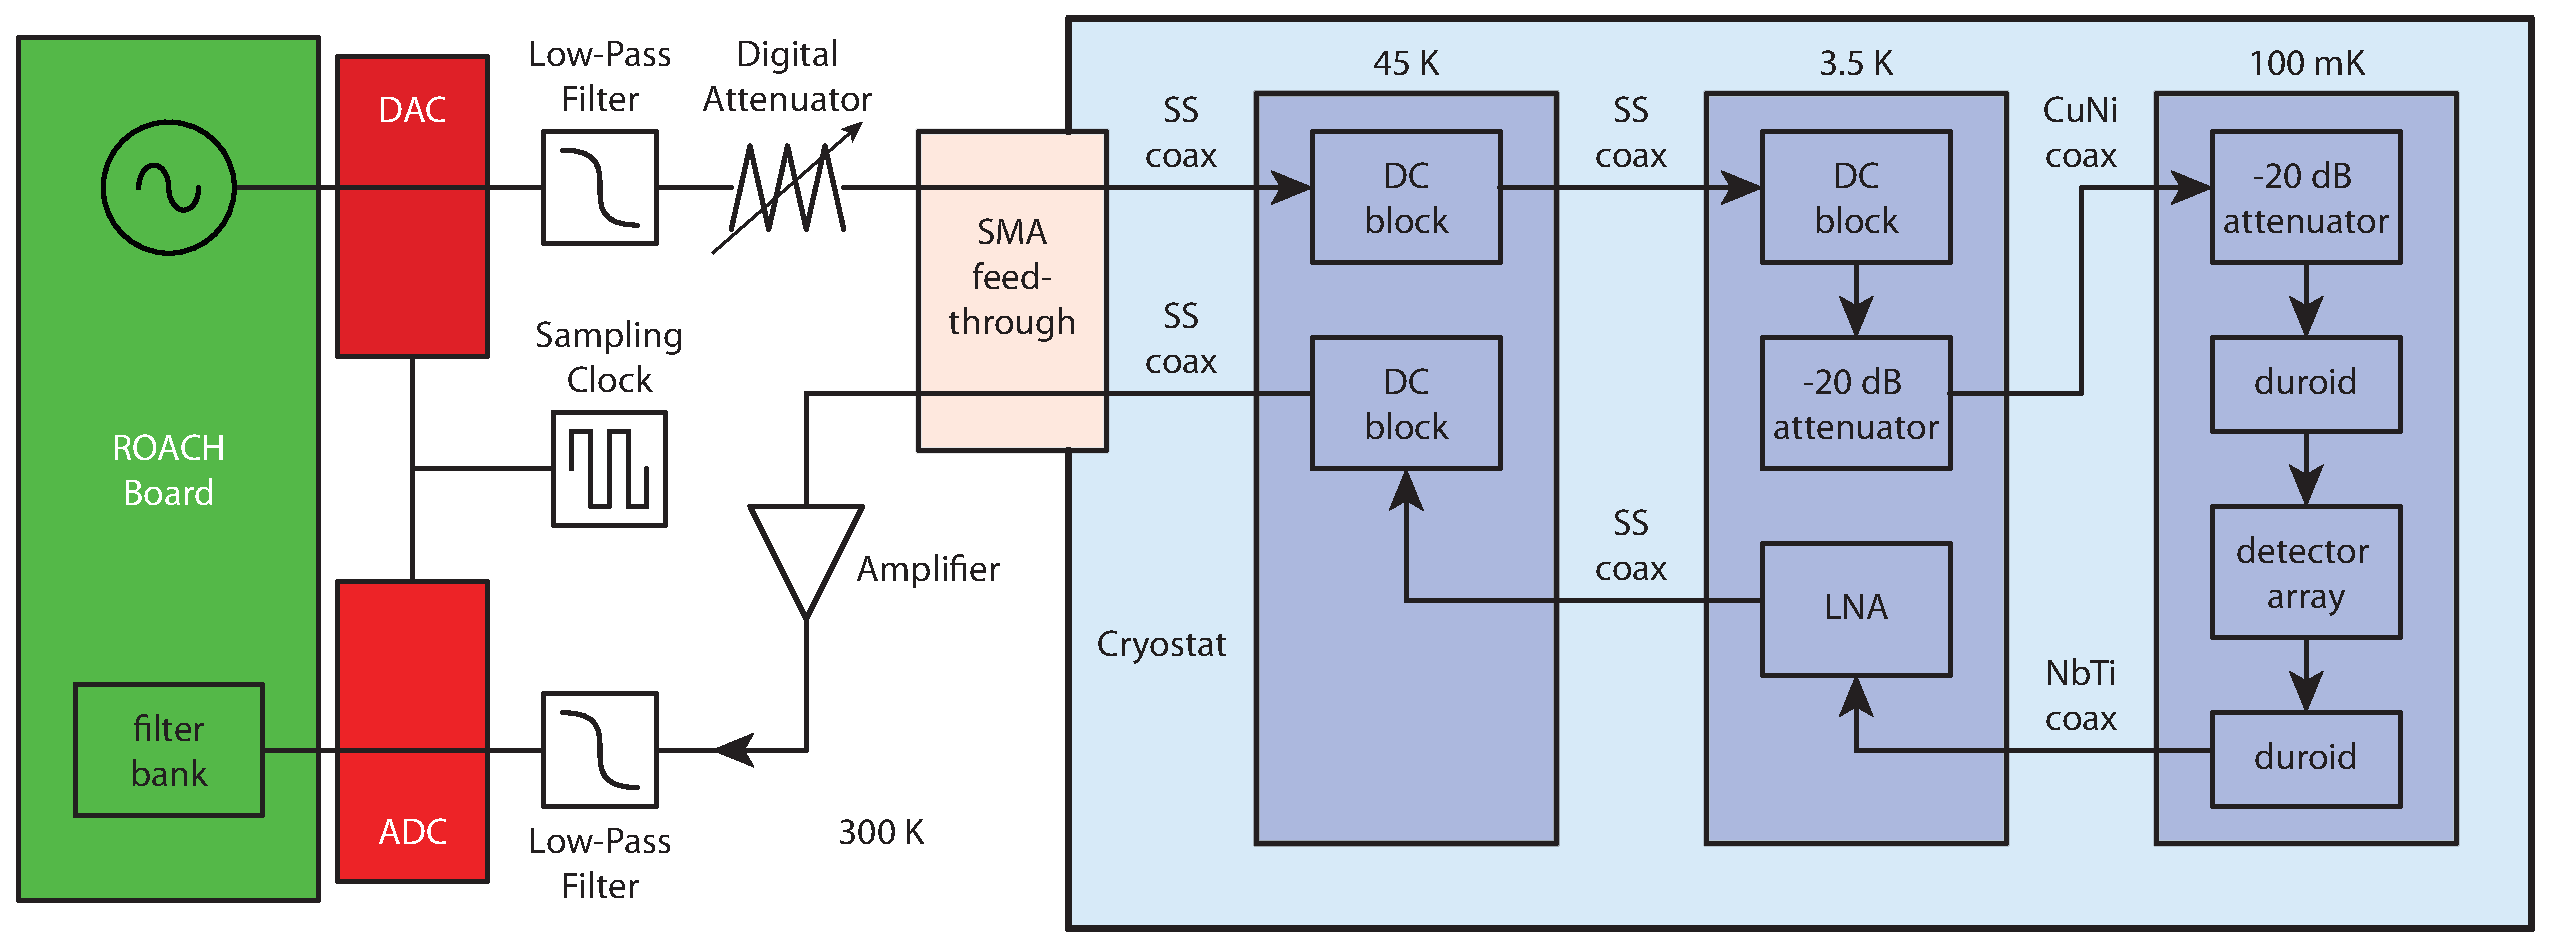
\includegraphics[width=0.8\textwidth]{hardware/baseband_readout_schematic.pdf}
\caption[A schematic of the ROACH-1 baseband readout system, including components in the cryostat.]
{
A schematic of the ROACH-1 baseband readout system, including components in the cryostat.
This system is capable of measuring resonances below approximately \SI{200}{MHz}.
This figure was published in \textcite{McCarrick2014RSI}.
}
\label{fig:baseband_readout_schematic}
\end{figure}

\begin{figure}[htb]
\centering
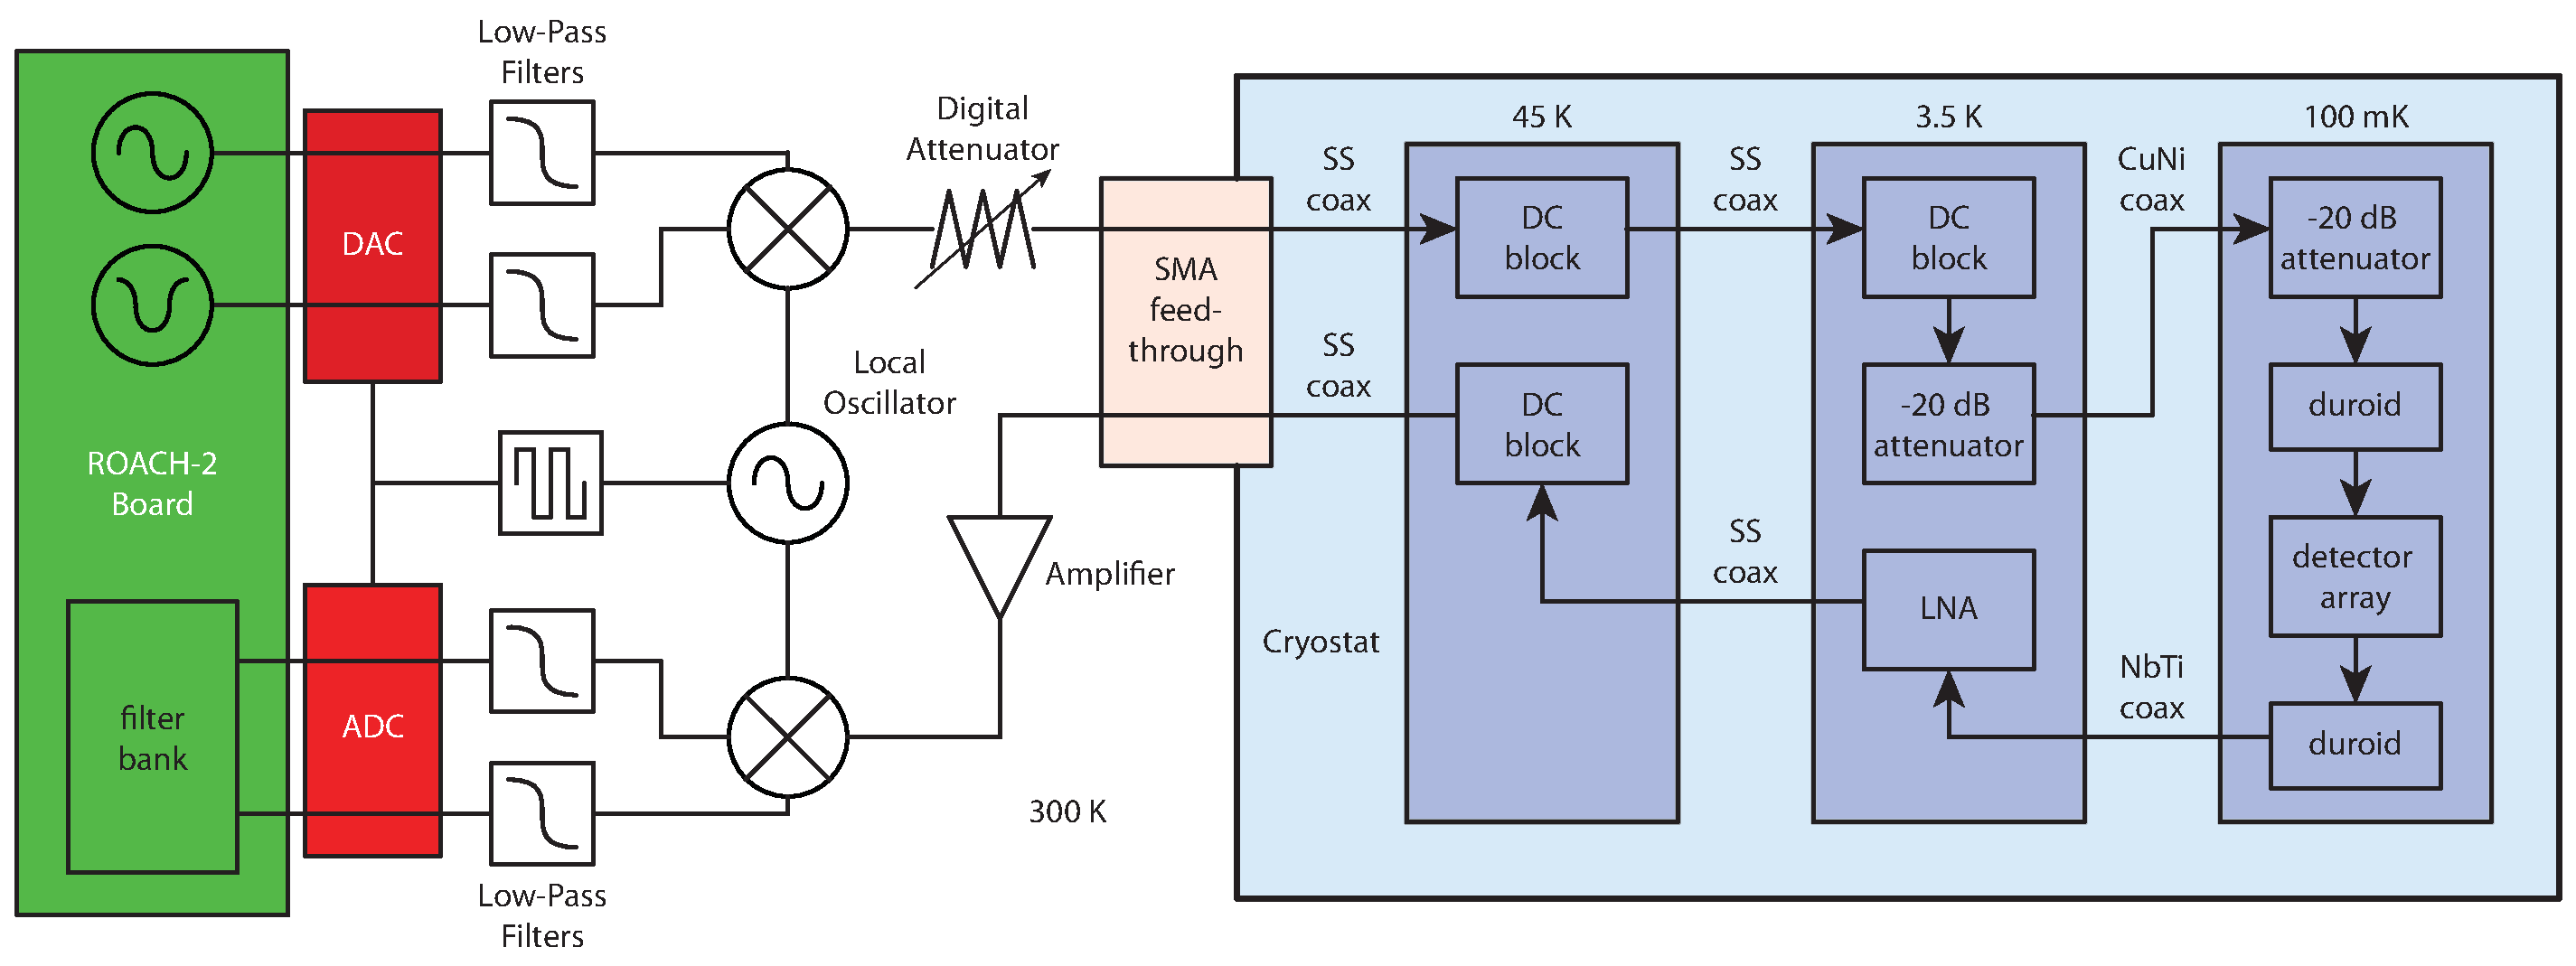
\includegraphics[width=0.8\textwidth]{hardware/heterodyne_readout_schematic.pdf}
\caption[A schematic of the ROACH-2 heterodyne readout system, including components in the cryostat.]
{
A schematic of the ROACH-2 heterodyne readout system, including components in the cryostat.
This system is capable of measuring resonances between approximately \SIrange{700}{4000}{MHz}.
This figure was published in \textcite{Johnson2016SPIE}.
}
\label{fig:heterodyne_readout_schematic}
\end{figure}

\begin{figure}[htb]
\centering
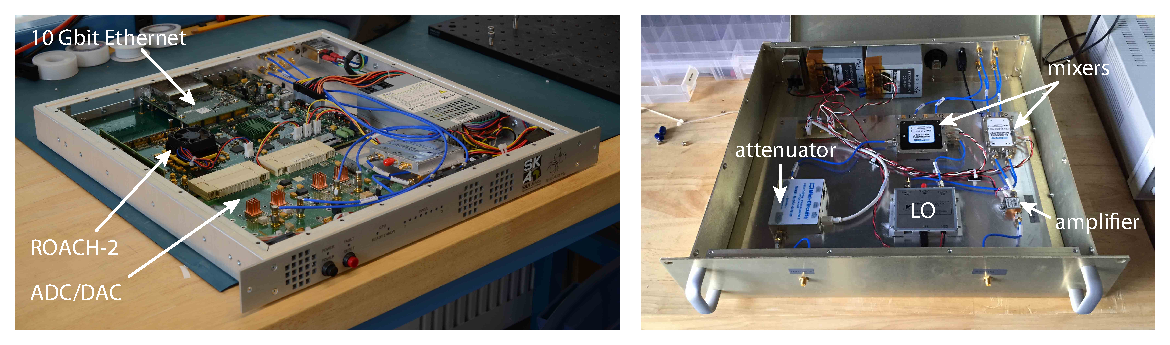
\includegraphics[width=\textwidth]{hardware/roach-2_v2.pdf}
\caption[Photographs of the ROACH-2 board and the heterodyne analog electronics box.]
{
\textbf{(Left)}
A photograph of the ROACH-2 board.
\textbf{(Right)}
A photograph of the analog electronics box for the heterodyne readout system, including the local oscillator (LO).
This figure was published in \textcite{Johnson2016SPIE}.
}
\label{fig:roach-2_v2}
\end{figure}

\clearpage


\section{Millimeter-wave source}
\label{sec:hardware.mmw_source}

\begin{table}[htb]
\centering
\caption[Primary components of the millimeter-wave source.]{Primary components of the millimeter-wave source.
The terminator and amplifiers are built-in components, but are used only in broadband mode, in which they produce broadband noise.
In continuous-wave mode, we instead use an external microwave signal generator that feeds the input to the PIN switch.}
\renewcommand{\arraystretch}{1.2}
\begin{tabular}{lll}
\toprule
\textbf{Component} & \textbf{Vendor} & \textbf{Part Number} \\
\midrule
50~$\Omega$ terminator & Minicircuits & ANNE-50X \\ 
High gain amplifiers & Spacek Labs & SG134-40-17 \\ 
PIN switch & Narda & S213D \\ 
Active multiplier & Millitech & AMC-05 \\
Variable attenuators & Custom Microwave & VA6R \\
Band-pass filter & Pacific Millimeter & 14020 \\
Directional coupler & Millitech & CL3-006 \\
Zero-bias diode power detector & Virginia Diodes, Inc. & WR6.5-ZBD \\
\bottomrule
\end{tabular}
\label{tab:mmw_source}
\end{table}

\begin{figure}[htb]
\centering
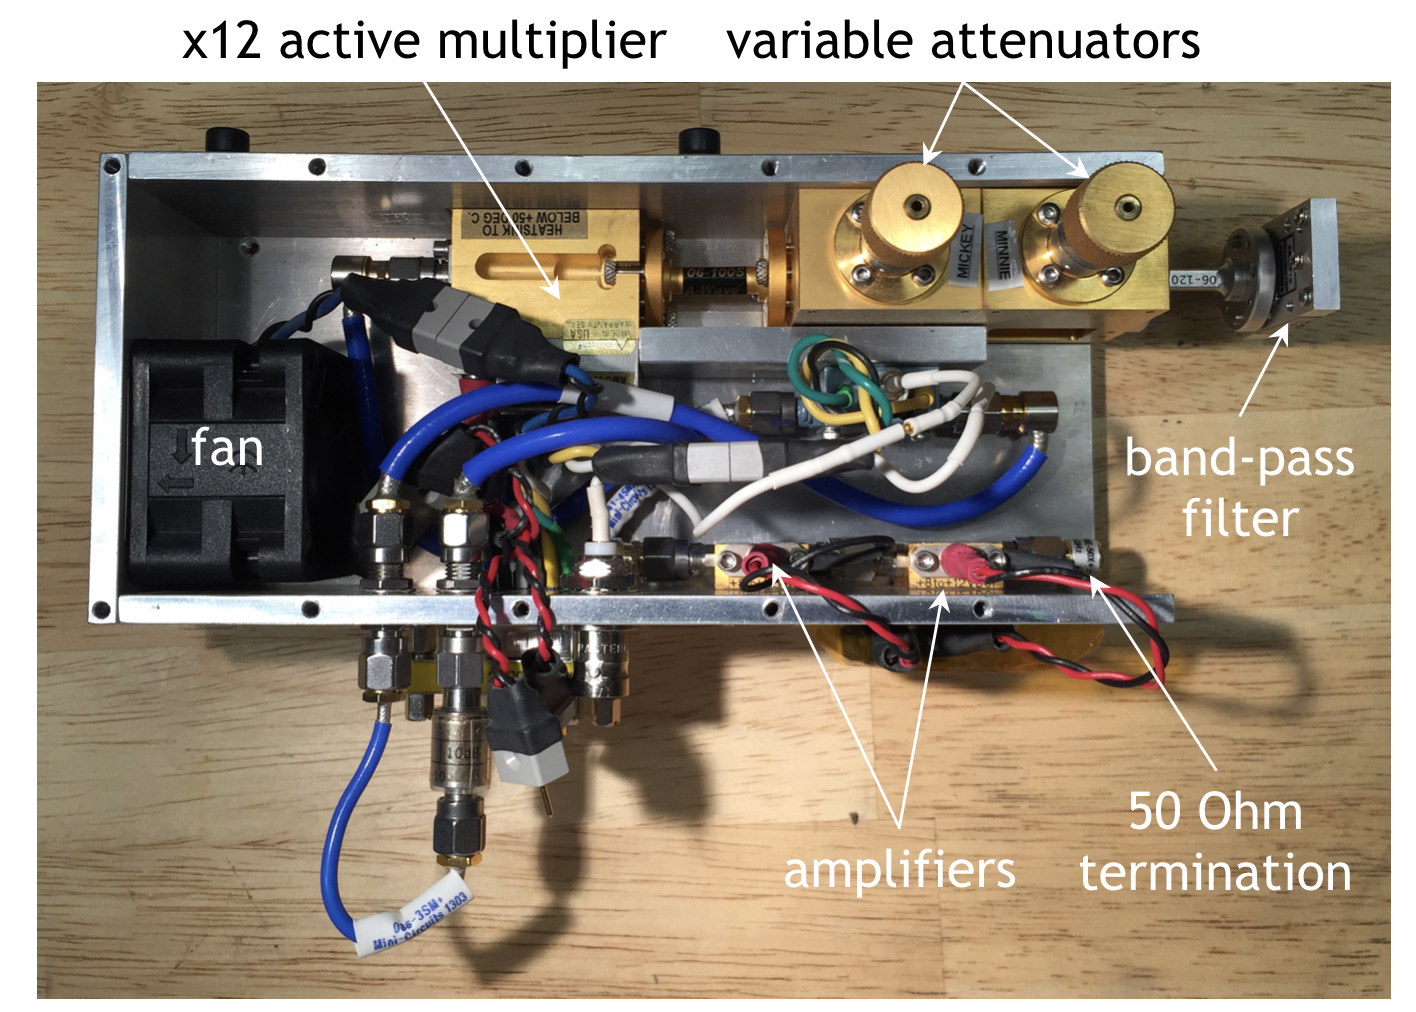
\includegraphics[width=0.7\textwidth]{hardware/millimeter-wave_source_annotated.png}
\caption[A photograph of the electronic millimeter-wave source.]
{
A photograph of the electronic millimeter-wave source.
}
\label{fig:millimeter-wave_source_annotated}
\end{figure}

\clearpage

\begin{comment}
\section{Package for multichroic detectors}
\label{sec:hardware.package}

\todo[inline]{Describe the multichroic detector package.}
The upper piece, the \textit{holder}, includes the feedhorns and waveguides, structures used to align the wafer, and 
The lower piece, the \textit{lid}, closes the module and contains backshorts that improve the millimeter-wave coupling.

\begin{figure}[htb]
\centering
\missingfigure[figwidth=\textwidth]{Lots of pictures of the multichroic package.}
\caption[Pictures of the multichroic package.]
{Pictures of the multichroic package.}
\label{fig:multichroic_package}
\end{figure}

\clearpage
\end{comment}

\section{Cryostat}
\label{sec:hardware.cryostat}

\begin{figure}[htb]
\centering
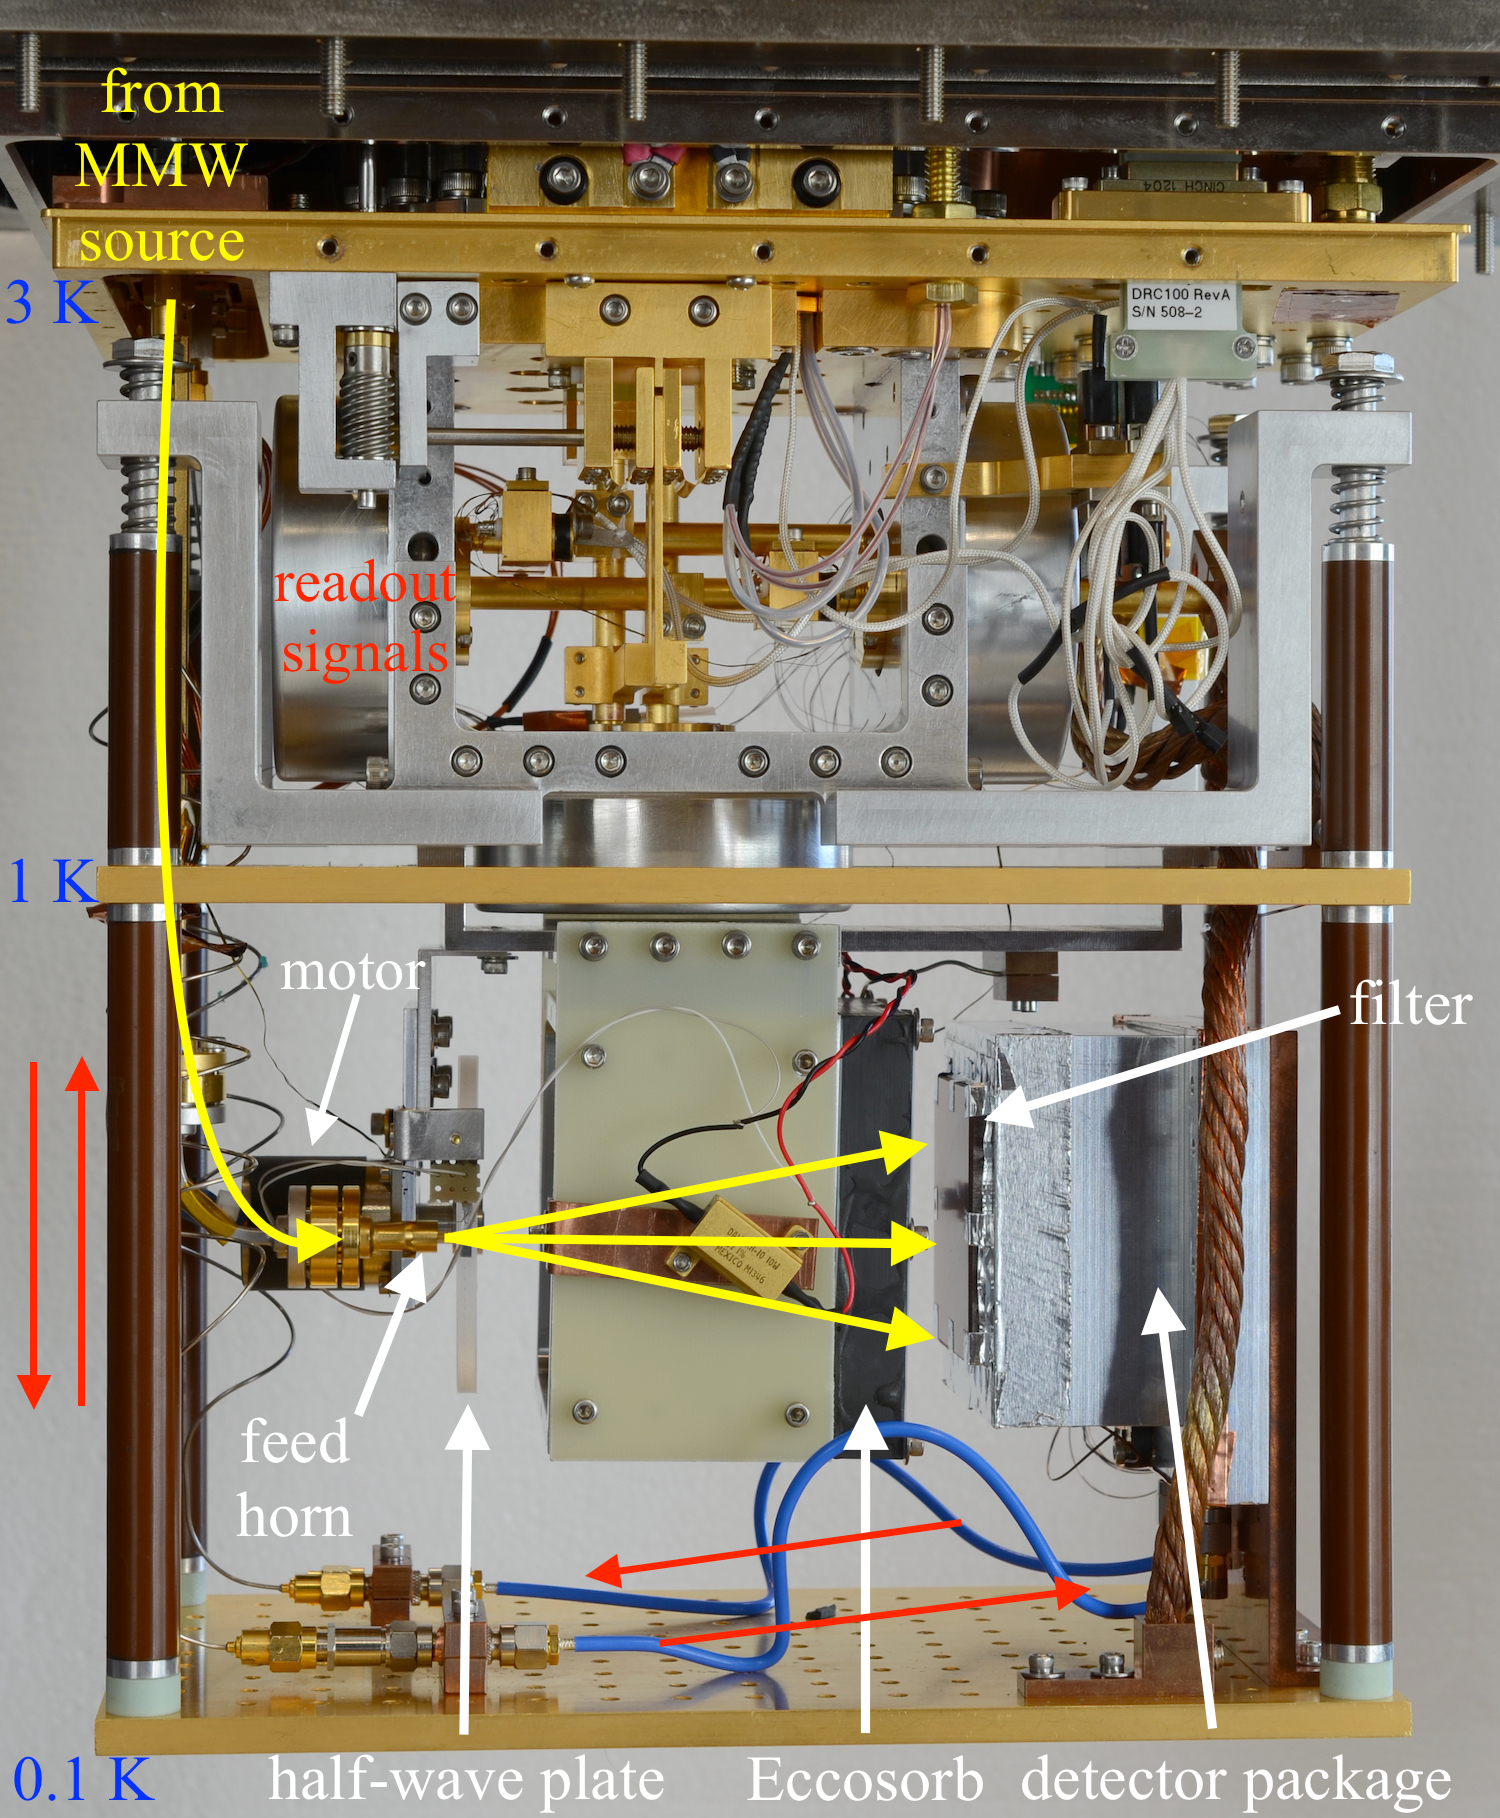
\includegraphics[height=0.7\textheight]{hardware/starcryo_cryostat_with_hwp.jpg}
\caption[The interior of a cryostat used for detector testing, in its ``half-wave plate'' configuration.]
{
The interior of a cryostat used for detector testing, in its ``half-wave plate'' configuration.
Light from an electronic millimeter-wave source propagates down the rectangular waveguide and exits the feed horn.
The cryogenic half-wave plate may rotate the polarization axis.
The motor rotates the half-wave plate.
The Eccosorb slab is nearly opaque and provides a beam-filling black body load with a temperature that can be controlled using the heater.
This configuration is similar to that used for the optical testing of detectors described in Section~\ref{sec:multichroic.mkidarray02}.
}
\label{fig:starcryo_cryostat_with_hwp}
\end{figure}

\begin{figure}[ht]
\centering
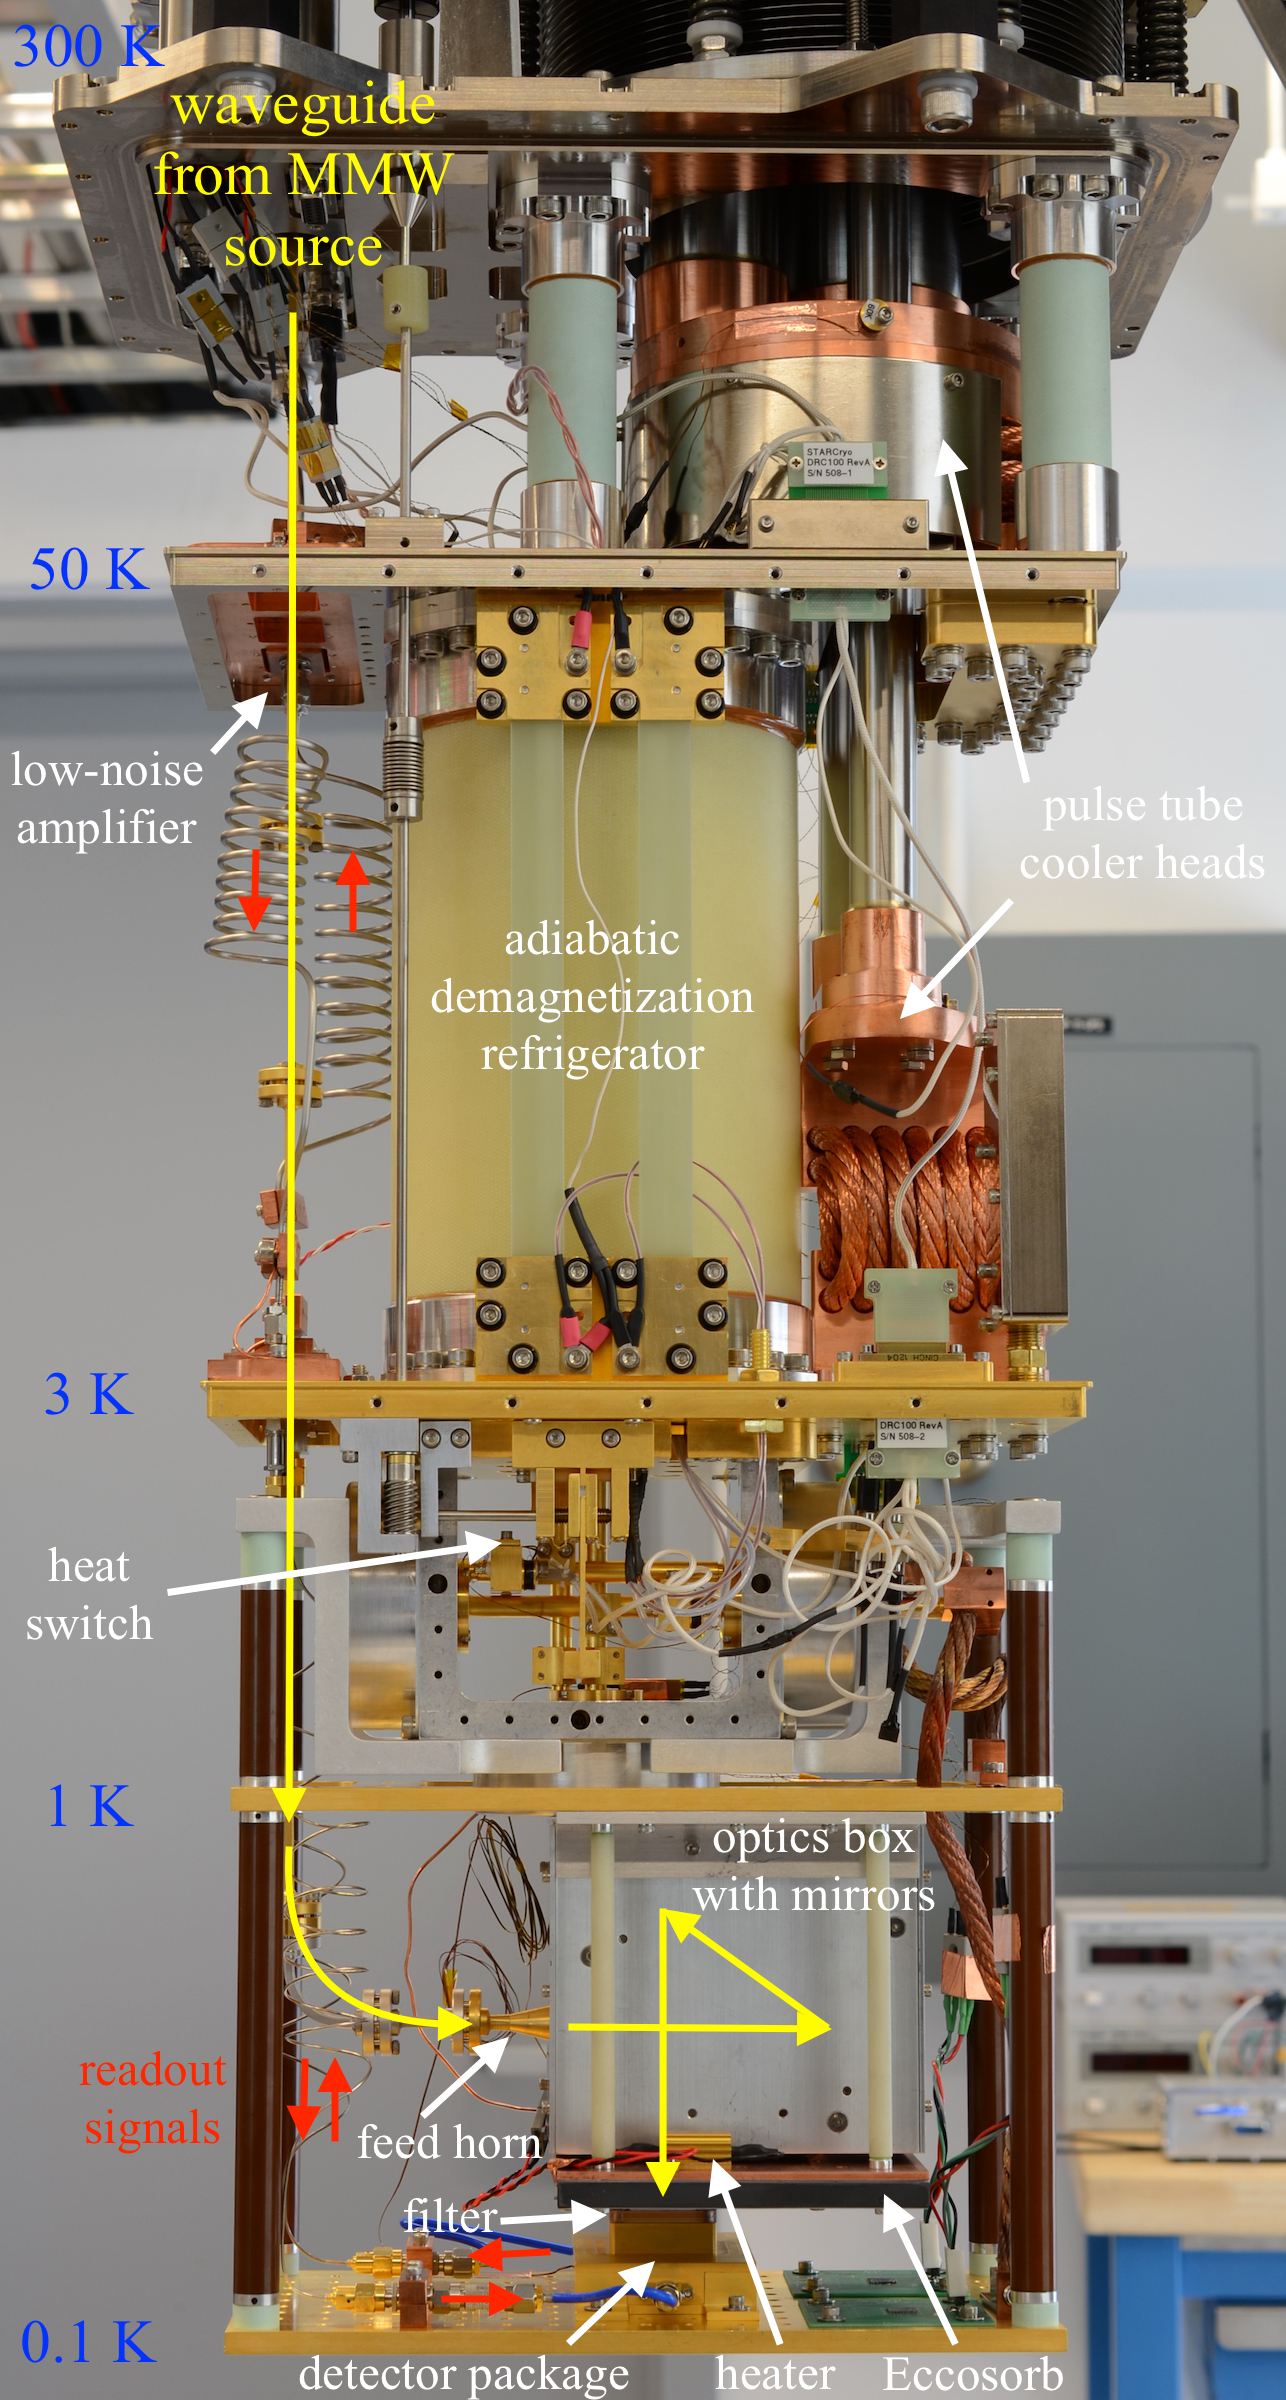
\includegraphics[height=0.8\textheight]{hardware/starcryo_cryostat_with_optics_box.jpg}
\caption[The interior of a cryostat used for detector testing, in its ``optics box'' configuration.]
{
The interior of a cryostat used for detector testing, in its ``optics box'' configuration.
Light from an electronic millimeter-wave source propagates down the rectangular waveguide and exits the feed horn.
The optics box contains mirrors (not visible) that convert the horn beam into a plane wave that illuminates the top of the detector package.
The Eccosorb slab is nearly opaque and provides a beam-filling black body load with a temperature that can be controlled using the heater.
The experiment described in Section~\ref{sec:sensitivity.measuring} used a similar configuration to that shown here.
The experiment described in Section~\ref{sec:loss.vortex} was performed with the package attached to the \SI{0.1}{K}, as shown here, but the optics box was removed and the magnet array was placed beneath the package, outside the cryostat shells that have been removed for this photograph.
}
\label{fig:starcryo_cryostat_with_optics_box}
\end{figure}

